\chapter{Traceability and Provenance}
\label{sec:trace}

The technologies in the INTO-CPS tool chain are able to automatically capture traceability information as activities are performed using the various parts in the tool chain. This includes information about who created or modified an artefact (model, simulation result etc.) and which requirements it is linked to. The traceability features of the INTO-CPS tool are powerful, but require a specific workflow to be followed in order to make best use of them. This chapter explains the steps in this workflow.

This chapter appears first in this advanced material as the following chapters, in particularly Chapters~\ref{sec:reqeng} and~\ref{sec:sysml}, provide key guidance on the first part of the workflow that must be followed in order for traceability to be realised. Those not wishing to use the traceability features can read chapters in any order, driven by their needs or interest. This chapter should be used in conjunction with the User Manual (Deliverable D4.3a~\cite{INTOCPSD4.3a}), which covers details of how to enable traceability recording in the INTO-CPS Application and baseline tools\footnote{Traceability is turned off by default as it can be intrusive if the right workflow is not followed.}. Readers interested in detailed specifications of the traceability and provenance features are directed to Methods Progress Report (Deliverable D3.3b~\cite{INTOCPSD3.3b}), while the tool implementation is described in Deliverables D4.2d~\cite{INTOCPSD4.2d} and D4.3d~\cite{INTOCPSD4.3d}.


\section{Traceability Workflow}

The INTO-CPS tool chain builds a graph of traceability relations, as there can be multiple relationships between different artefacts. The graph is however tree-like in the sense that there must be some root node(s) to trace from or back too. These root nodes are \emph{requirements}. To use fully the machine-assisted traceability features, it is necessary to initialise the traceability graph by using Modelio from the beginning of the development process. This means that it is necessary to follow these steps:

\begin{enumerate}[noitemsep]
  \item Define requirements through some requirements process (see guidance in Chapter~\ref{sec:reqeng});
  \item Create a Requirements Diagram (RD) in Modelio representing these requirements;
  \item Create an Architecture Structure Diagram (ASD) and Connections Diagram (CD) describing the multi-model;
  \item Link each requirement to one \texttt{<<EComponent>>} (FMU);
  \item Export model descriptions for each \texttt{<<EComponent>>};
  \item Import model descriptions into baseline tools; and
  \item Generate a multi-model configuration from the CD.
\end{enumerate}

After these steps, the traceability graph will then be updated by the baseline tools as models are created from the model descriptions, FMUs are exported and so on, and co-simulation runs and results will be recorded by the INTO-CPS Application. Therefore, by following this workflow it is possible to take advantage of the machine-assisted traceability within INTO-CPS. By performing the required manual input of requirements and links to SysML elements, it is then possible to automatically trace forward to models, FMUs and simulation results, and to trace backwards from these artefacts to individual requirements.

\section{What Artefacts are Traced?}

%\draftnote{KGP: Our requirements said that we list traced artifacts, so we can quickly summarise the schema here perhaps?} 

%\draftnote{CJG: Start by introducing briefly PROV and OSLC relations, which are the basis of the traces}

Traceability in the INTO-CPS tool chain is based upon a study of the actions performed when using the INTO-CPS tool chain, the artefacts that are used and produced and a combination of two existing standards, the W3C's Prov~\footnote{\url{https://www.w3.org/TR/prov-overview/}} and the OMG's OSLC~\footnote{\url{http://open-services.net/}}.   The combination of these resulted in the INTO-CPS traceability ontology that captures in detail all elements in the INTO-CPS workflow and describes the relationships between them.  The complete ontology is presented in deliverable D3.3b~\cite{INTOCPSD3.3b} and a summary is presented here.

Traceability data is inherently a graph based structure based upon nodes and the connections between them, and Prov provides basic types for those nodes along with list of relationships that may exist between them.  The three types of nodes are: Entities, things that may be produced or used during a development process; Activities, are things that act upon and make use of entities; and Agents, objects that have responsibility for entities and activities.  The Prov relations then allow then connection of nodes such as an activity may use an entity, and an entity may be generated by an activity.  

The combination of the Prov nodes and relations supports the representation of the processes that lead to the generation of a particular entity, but it does not support connection of those entities to requirements.  OSLC contains a set of specifications, each of which defines a list of relations that it supports between entities. In the case of the INTO-CPS traceability, parts of the OSLC architecture management and requirements management specifications are employed, these allow the connection of entities to requirements via a 'satisfies' relation indicating the entity attempts to address the needs of the requirement, additionally it allows the connection of simulation results to requirements via a 'verifies' relation indicating that the requirement has been met.

%\draftnote{CJG: Introduce that we break the process down into almost atomic actions}

The INTO-CPS traceability ontology breaks the INTO-CPS workflow down into activities that, while not atomic if we consider a user's interaction with a particular tool, could be considered atomic when viewing the process of developing a CPS.  Figure~\ref{fig:traceability:step02} shows the traceability links recorded during one step in the development of a line following robot.  In this example, the requirements, R1 \& R2, already exist in the architecture models and the user has created an ASD to decompose the proposed robot into components.  The user has, at the same time, associated the blocks within the ASD with the the requirements that each block aims to satisfy.  When the user saves the updates architecture model, the Modelio tool records the user's 'Architecture Modelling' activity, along with references to the ASD, the blocks it contains and the newly created links between the blocks and the requirements.  Here the \emph{used}, \emph{wgb} (short for 'was generated by'), \emph{assoc} (short for 'associated with') and \emph{attrib} (short for 'attributed to') are links that come from the Prov standard.  The \emph{OSLC\_Sat} (short for 'satisifies') comes from the OSLC requirements management specification.

%\draftnote{CJG: Give example of one action in detail}

\begin{figure}[htbp]
	\centering
	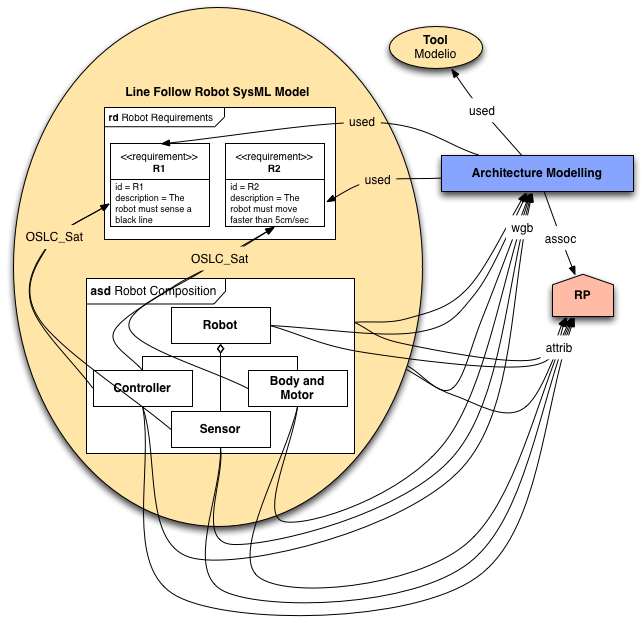
\includegraphics[width=0.8\textwidth]{figures/Traceability/step02}
\caption{Traceability links captured during the production of an ASD for a line following robot.}\label{fig:traceability:step02}
\end{figure}

%\draftnote{CJG: As the user(s) use the tools, they each record the their atomic actions, forming the traceability graph}

A development project will likely consist of many instances of the activities identified in the ontology being performed and together they form a traceability graph.  Figure~\ref{fig:traceability:abstractTraceFlow} shows a simplified view of a traceability graph with some steps removed for brevity.  At the top of the graph we see the architecture modelling step described previously, that produces an architecture model.  From the architecture, model description files are exported to start the production of the simulation models.  In turn the simulation models are exported as FMUs and the FMUs are used to produce simulation results.  Key to the traceability graph then are the 'used' and 'wgb' connections that can be used by a query to determine from where each entity was generated.  By following these links back from any entity to the individual blocks within the architecture model, it is possible to determine which requirement(s) each should satisfy.  Finally when simulation results are output, these may be linked back to the relevant requirements, stating whether a requirement was verified or violated by that result.

%\draftnote{CJG: Give abstract view of a resulting trace}


\begin{figure}[htbp]
	\centering
	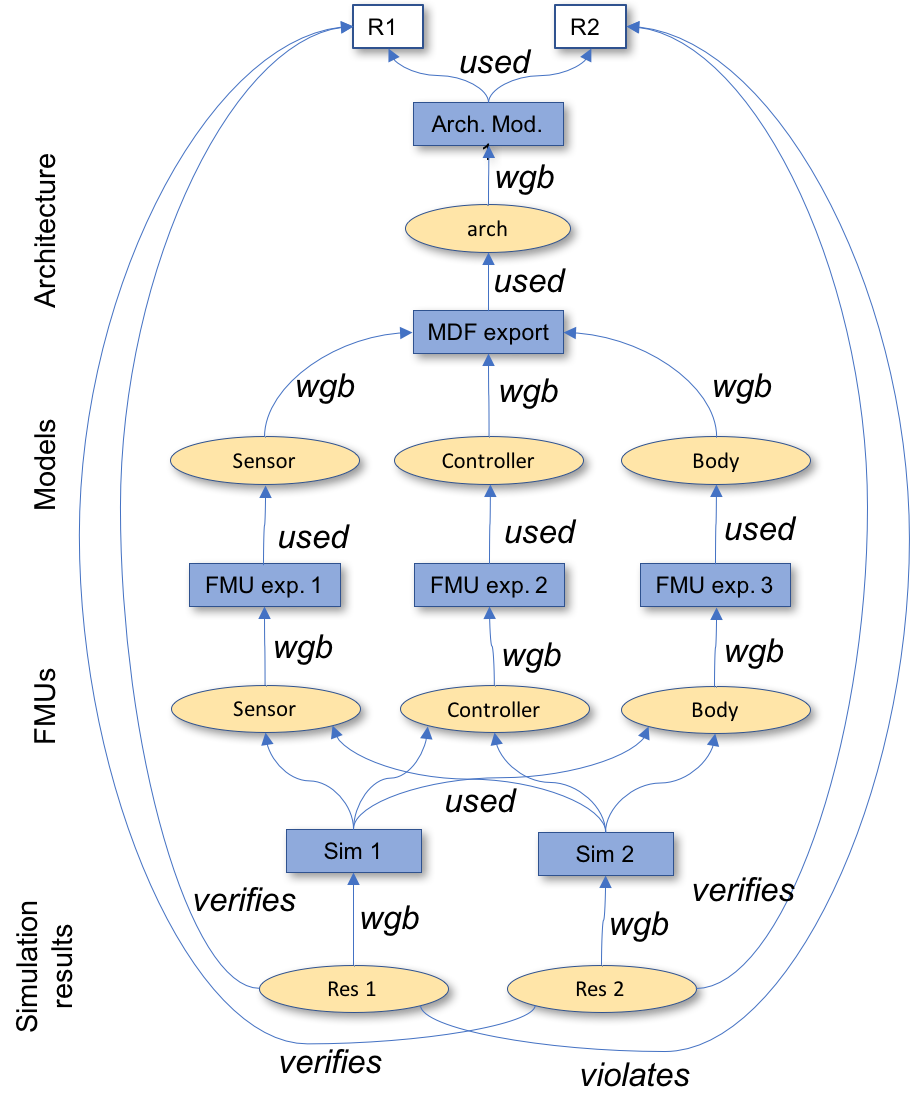
\includegraphics[width=0.7\textwidth]{figures/Traceability/abstractTraceFlow}
\caption{Traceability links captured during the production of an ASD for a line following robot.}\label{fig:traceability:abstractTraceFlow}
\end{figure}


%\draftnote{CJG: A paragraph outlining the entities, activities and agents}

The traceability ontology captures the significant activities and entities that form the INTO-CPS workflow.  For example a development project might see the following activities recorded in the traceability graph:  \emph{Requirements Management}, \emph{Architecture Modelling}, \emph{Architecture Configuration Creation} \emph{Model Description Export}, \emph{Simulation Modelling}, \emph{FMU Export}, \emph{Configuration Creation}, \emph{Simulation Configuration Creation} and then \emph{Simulation}.  These activities are connected in the workflow by the entities they create and use, so the example would see the traceability graph containing records of: \emph{Archtecture Structure Diagram}, \emph{Architecture SubSystem}, \emph{Architecture Connection Diagram}, \emph{Model Description File}, \emph{Simulation Model}, \emph{FMU}, \emph{Multi-model Configuration}, \emph{Simulation Configuration} and \emph{Simulation Result}.  Alongside these will be records of the agent(s), who are both associated with activities and have entities attributed to them. 



\section{Traceability Queries}

%\draftnote{TWT: FMU -> Requirements and Simulation Results -> FMUs are currently implemented.}

The traceability graph created by the INTO-CPS tool chain uses a graph database tool called \emph{Neo4J}. Once a graph has been built, queries can be executed over the graph to perform both forwards and backwards traceability. Below are some types of queries that can be executed over the graphs. The INTO-CPS Application supports some of these queries with the GUI, and the rest through inline access to the Neo4J console.

\begin{enumerate}[noitemsep]
  \item Impact analysis
  \begin{itemize}
    \item Forward traceability (from requirements to entities)
    \item Backwards traceability (from FMU to requirements)
    \item Backwards traceability (from components to requirements)
  \end{itemize}
  \item Simulation sources
  \begin{itemize}
    \item Find all simulations
    \item Find sources and sinks for a simulation
  \end{itemize}
  \item Coverage
  \begin{itemize}
    \item Requirements without architecture elements
    \item Requirements without simulation models
    \item Requirements without FMUs
    \item Requirements without positive simulation results
    \item Requirements without any simulation results
  \end{itemize}
  \item Code sources
  \begin{itemize}
    \item Find all generated source code entities
    \item Find the models for a given source code entity
  \end{itemize}
  \item User impact
  \begin{itemize}
    \item Find all users in the database
    \item Find all artefacts influenced by a user
    \item Find all activities performed by a user
  \end{itemize}
\end{enumerate}

Queries are written in Cypher, a query language built into Neo4J. Advanced users or those developing extensions to INTO-CPS can build their own queries in Cypher\footnote{\url{https://neo4j.com/developer/cypher-query-language/}} and execute them using Neo4J directly as described in the User Manual (Deliverable D4.3a~\cite{INTOCPSD4.3a}). 